\documentclass{standalone}

\usepackage{amsmath,amsfonts,amssymb,amsthm,mathtools} 
\usepackage{fontspec}            % пакет для подгрузки шрифтов
\setmainfont{Burst My Bubble}   % задаёт основной шрифт документа

% why do we need \newfontfamily:
% http://tex.stackexchange.com/questions/91507/
\newfontfamily{\cyrillicfonttt}{Burst My Bubble}
\newfontfamily{\cyrillicfont}{Burst My Bubble}
\newfontfamily{\cyrillicfontsf}{Burst My Bubble}
% Иногда тех не видит структуры шрифтов. Эти трое бравых парней спасают ситуацию и доопределяют те куски, которые Тех не увидел.

\usepackage{unicode-math}     % пакет для установки математического шрифта
\setmathfont{Asana Math}      % шрифт для математики

\usepackage{polyglossia}      % Пакет, который позволяет подгружать русские буквы
\setdefaultlanguage{russian}  % Основной язык документа
\setotherlanguage{english}    % Второстепенный язык документа

\usepackage{pgf,tikz,pgfplots}
\usetikzlibrary{arrows,calc}
\usepackage{relsize} 

\usepackage{graphicx} 
\usepackage{rotating}
\usepackage{xcolor}
\usepackage{color}
\usepackage{minted}

%\newcommand{\Big}{\fontsize{50}{60}\selectfont Foo}

\definecolor{catcolor}{HTML}{DBC0A5}

\begin{document}

\begin{tikzpicture}[scale=2]

% Cat
\node[inner sep=0pt] (russell) at (-0.3,-0.8) {
\includegraphics[angle=0,scale=0.2]{cat.png}};    

% plantain
\node[inner sep=0pt] (russell) at (0.8,0.6) {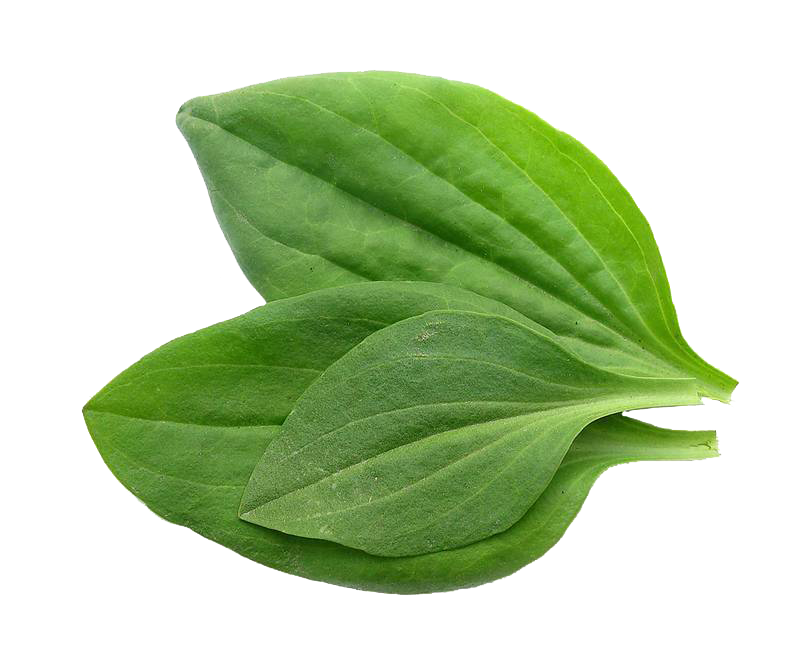
\includegraphics[angle=-30,scale=0.12]{plantain.jpg}};    

\begin{scope}[rotate=30]   
% Radius of regular polygons
  \newdimen\R
  \R=2cm
  \coordinate (center) at (0,0);
 \draw (0:\R)
     \foreach \x in {60,120,...,360} {  -- (\x:\R) }
              -- cycle (300:\R)
              -- cycle (240:\R)
              -- cycle (180:\R)
              -- cycle (120:\R)
              -- cycle (60:\R)
              -- cycle (0:\R)  [line width=3.8pt,color=catcolor];
\end{scope}       
       
% Matrix              
\draw[color=black,draw,align=left] (-0.97,0.8) node[right] { 
\mint{python}|import this|
%\begin{minted}{R}
%if( 0.4-0.3 == 0.1 ){
%	print("всё хорошо")
%}
%\end{minted}
};       

\end{tikzpicture}

\end{document}